\chapter{Priorização dos Esforços}
\label{cap-esforcos}

    \begin{figure}[htbp!]
        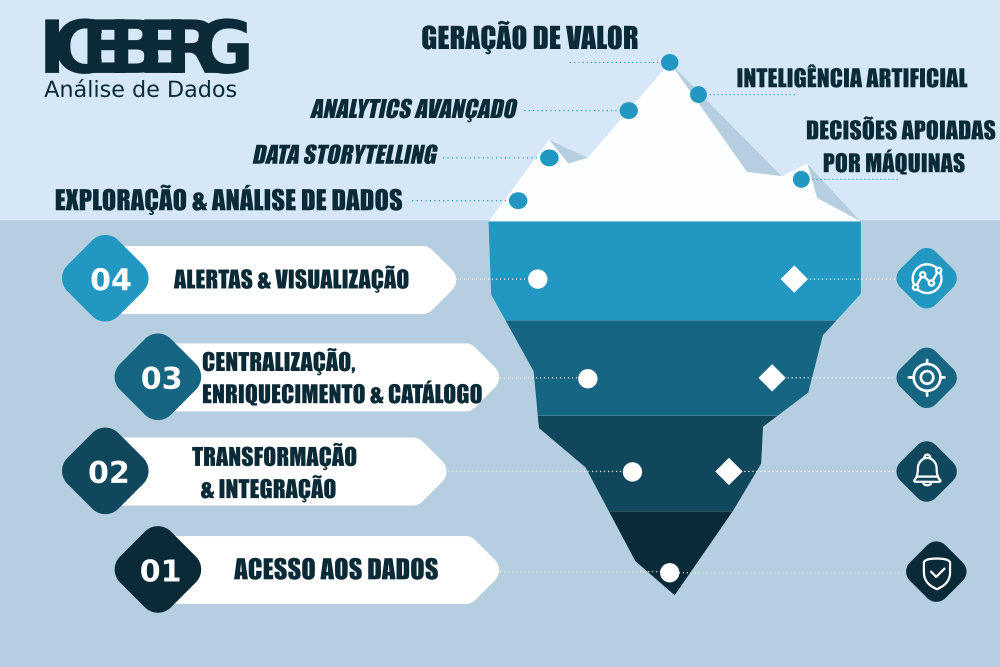
\includegraphics[width=\textwidth]{fig/fig-iceberguebi.png}
        \caption{O Iceberg da análise de dados. Fonte: Elaboração própria.}
        \label{fig:icebergbi}
    \end{figure}
    
A figura \ref{fig:icebergbi} apresenta um infográfico contendo o panorama de uma implantação de sucesso de um ambiente de análise de dados em uma organização. Na superfície encontra-se a parte visível do iceberg representando os recursos desejados pelos gestores e altos executivos de uma organização. Abaixo da superfície encontra-se a parte invisível, que dá sustentação à porção visível.

É essencial se ter em mente que não há como se obter os valores vistos nas camadas superiores sem que haja a respectiva sustentação das camadas inferiores. Assim, é precipitado se começar um projeto de ambiente de análise de dados investindo-se nas tecnologias que aparecem na superfície do iceberg, mas esquecendo-se de empreender esforços nas atividades que darão sustentação a esse ambiente. 

Dessa forma, nesse capítulo, vamos aproveitar a figura do iceberg para propor a ordem correta de ações e investimentos para que seja possível alcançar a geração de valor almejada pela organização.

\section{Acesso aos Dados}

No caso específico da CLDF sobre o qual se estuda, que cria o projeto no âmbito da atividade de fiscalização do Poder Legislativo, os dados brutos são exatamente os dados do ente fiscalizado, sobre os quais deseja-se extrair os valores. A título de exemplo, no caso de se buscar aferir uma correlação entre denúncias do \emph{disque-denúncia} e posterior prisão dos denunciados, então deve-se obter dados do sistema do \emph{disque-denúncia}, bem como dados do sistema prisional. Esses dados encontram-se sob gestão dos órgãos que atuam nesses sentidos, e não do órgão fiscalizador.

Para isso, faz-se necessário que o órgão fiscalizador acesse esses dados, para então usá-los como insumo. Este acesso pode ser feito conforme as maneiras que podem ser vistas na seção \ref{acessos-dados}.

Vale lembrar que a falta do devido acesso e estratégia de captura de dados pode levar a um esvaziamento do repositório analítico, que compromete a geração de valor de todo o investimento feito na solução. Por esse motivo, o acesso aos dados é essencial de ocorrer como primeiro passo, para que não se incorra no pior cenário da seção \ref{sub-cenario-naotemosingredientes} do Capítulo \ref{cap-descricao} ``\nameref{sub-cenario-naotemosingredientes}'' na qual um investimento alto é realizado e, por outro lado, a solução não agrega valor para a organização.

%\TODO{INFORMAR CAPÍTULO DE ARQUITETURA PROPOSTA}

\section{Transformação e Integração}
\index{Transformação}
\index{Integração}

A transformação e integração de dados é melhor detalhada de uma forma geral na subseção \ref{acessos-dados}. No caso específico da CLDF, a transformação e integração são atividades simples para as primeiras iterações que serão realizadas. Para este primeiro momento, uma solução simples de desenvolvimento interno pode já ser suficiente para cumprir com este requisito; porém, conforme houver novas iterações de novos dados coletados, com maior complexidade, será necessário o uso de uma solução corporativa, para as quais existem tanto ferramentas livres como licenciadas.

É muito importante que a equipe que implementar os algoritmos de transformação tenha em mente as padronizações de dados que serão utilizadas, sempre visando a melhor adequação à necessidade da CLDF. Na fase da transformação, devem ser também tomados os cuidados para que os dados sejam tratados em conformidade com a Lei Geral de Proteção de Dados -- LGPD.

Ao fim, para a realização da integração, deve-se manter clara e documentada a estratégia de integração, se será completa ou incremental, bem como verificar a melhor adequação às bases utilizadas na camada de armazenamento analítico. Para a integração, é importante que sejam adotadas boas práticas para o carregamento de dados em lote em um SGBD, usando dos recursos disponibilizados pela ferramenta.

\section{Centralização, Enriquecimento, Catálogo}
\index{Centralização}
\index{Enriquecimento}
\index{Catálogo}

Os passos de centralizar, enriquecer e catalogar encontram-se detalhados nas subseções \ref{sec:centralizar}, \ref{sec:enriquecer} e \ref{sec:catalogar}, respectivamente. No caso específico da CLDF, esses passos não devem ser vistos como necessários para atendimento da primeira entrega, relacionada ao primeiro painel ou alerta gerado.

Entretanto, vale ressaltar o fato de que a existência de um catálogo na CLDF contribuirá para uma melhor eficiência do serviço, tendo-se em vista que o catálogo é essencial para se aproveitar um uso \emph{self-service} na montagem de painéis e alertas, aumentando a eficiência do usuário, bem como contribuindo para uma diminuição do nível de especialidade necessário, permitindo, inclusive, a criação de visualizações pelos próprios clientes. Assim sendo, é de grande importância que o catálogo seja implementado, ainda que não na primeira iteração.

A centralização dos dados, por sua vez, faz-se de grande necessidade para que seja realizada uma governança adequada sobre os dados, especialmente no tocante à adequação à Lei Geral de Proteção de Dados -- LGPD, além de otimizar os esforços do pessoal que for criar as visualizações, contribuindo também para o princípio da eficiência. A centralização é de implantação obrigatória; porém, não se mostra necessária já na primeira iteração.

O enriquecimento, por sua vez, permite ampliar o valor entregue ao cliente, permitindo a complementação das informações, de modo a gerar visualizações mais completas e autoexplicativas, sendo altamente recomendável de ser implantada.

\section{Alertas \& Visualização}
\index{Alertas}
\index{Visualização}

Para se gerar alertas e painéis de visualização, é necessário que haja uma ferramenta específica para esse fim. Os fornecedores estudados neste estudo possuem soluções robustas para entrega deste valor. A implantação da ferramenta, portanto, é essencial para o projeto de BI ser bem-sucedido.

Entretanto, para que se possa efetivamente fazer bom uso de uma dessas ferramentas, deve haver primeiramente estabelecidos os valores apontados pelas camadas inferiores, conforme citados nas seções anteriores. Havendo um repositório adequado de dados analíticos, torna-se simples a construção de painéis e alertas que agregam grande valor para qualquer organização, tanto pública como privada.

No universo das ferramentas de alerta e visualização, existem inúmeras, tanto abertas como licenciadas. É importante, no entanto, que a utilização seja feita buscando sempre uma padronização que torne simples a migração para uma nova ferramenta, já que os dados e painéis tendem a ser mais duráveis do que o ciclo de vida de uma ferramenta específica em uma organização.

\section{Analisar, Aprender, Otimizar}
\label{sec-aao}
\index{Analisar}
\index{Aprender}
\index{Otimizar}

A análise é melhor detalhada na subseção \ref{sec:analisar}. Em um primeiro momento, vislumbra-se uma análise feita por um usuário que possua um painel montado numa ferramenta para auxiliá-lo. Ademais, também vislumbra-se de imediato a geração de alertas, que já comportam um certo nível de análise automatizada. Percebe-se que o nível de automatização da análise é, portanto, pequeno na implantação inicial.

Entretanto, à medida em que surgirem mais projetos e o nível de complexidade desses seja crescente, o que é visto como um evento natural, o nível de automatização de análises tenderá a crescer, adentrando-se nos passos de aprendizado e otimização, melhor descritos nas subseções \ref{sec:aprender} e \ref{sec:otimizar}, respectivamente.

Cumpre destacar que é neste passo que o \emph{iceberg} mostrado na figura \ref{fig:icebergbi} começa a criar protuberâncias visíveis acima do nível da água. A trajetória passa então a exibir resultados exponenciais de valor, capazes de revolucionar o serviço atendido pela solução. No entanto, não é possível se pensar este valor sem se atender aos esforços mostrados nas seções acima, correspondentes às camadas inferiores do \emph{iceberg}.

Estes passos deverão ser pormenorizados em novo estudo, que é de grande importância que seja feito, uma vez que as camadas inferiores estejam satisfeitas, de modo a se estabelecer um percurso de implantação futuro. No entanto, destaca-se que muitas plataformas vendidas atualmente para a visualização já contam com recursos neste sentido.



% ##########################################
% ##########################################
% ##########################################
% ##########################################

\chapter{Implantação Ágil} 
\label{cap-proposta}
\index{Implantação}

Este capítulo propõe-se a apresentar uma proposta para a implantação de BI na CLDF. Para isso, é levada em consideração a realidade específica da CLDF, bem como a demanda por BI para auxiliar as Comissões no exercício do seu papel fiscalizador.

\section{Método Ágil}
\label{sec-metodoagil}
\index{Método Ágil}

Tendo-se em vista o arcabouço sobre projetos que existe atualmente, nos orientamos nas melhores e mais modernas práticas para sugerir que a implantação do BI na CLDF siga uma filosofia proveniente dos métodos ágeis. Agilidade é a capacidade de se adaptar a mudanças de requisitos, de equipe e de tecnologia. Um método ágil é necessário quando os requisitos e prioridades são instáveis, quando tanto o projeto e a construção são realizados simultaneamente ou quando durante o planejamento as fases de análise, projeto, implementação e testes não são tão previsíveis.

Trata-se, portanto, da implementação por funcionalidades, visando pequenas entregas que agreguem valor para o cliente final, com iterações incrementais e sucessivas.

O método ágil nasceu diante da insatisfação do mercado com o ritmo como os projetos estavam sendo tocados na grande maioria das organizações pelo mundo. O mundo atual apresenta um nível de dinamismo sem precedentes, e por esse motivo, muitos dos projetos acabavam finalizando sem fazer sentido, pois o contexto do momento de sua finalização era absolutamente diferente daquele do momento da sua concepção. Essa falta de sentido percebida levava também ao questionamento sobre a viabilidade econômica dos projetos, pois a percepção de valor tornava-se muito baixa para um alto investimento feito, e isso só era percebido depois que quase todo o investimento já havia sido dispendido.

Tendo-se em vista esse cenário, ocorreram diversas iniciativas no mundo corporativo para criar uma nova forma de fazer as coisas. Nisso destacam-se o Manifesto Ágil, no âmbito da Engenharia de Software, o Modelo \emph{Lean Startup} na criação de negócios, dentre outros \cite{prikladnicki2014}.


% não coloquei referencias direito pela falta de tempo, mas se tiver oportunidade, vou incluir

Uma das fortes premissas do modelo ágil é assumir a possibilidade de erros e valorizar a validação das hipóteses, que deve ser feita com a maior proximidade possível ao cliente final, que é o principal autor na percepção do valor gerado. Nesse sentido, deve-se buscar fazer com que os investimentos sejam feitos de forma gradual e aumentada à medida em que a proposta de valor esteja mais e mais validada.


\section{Metodologia Proposta}
\label{sec-implantacao}

No caso específico apresentado, sugerimos que sejam eleitas pequenas entregas de valor para os clientes finais, e que a ordem do projeto siga essa sequência, à medida do possível. 

Nesse sentido, primeiramente deve-se estabelecer a seguinte sequência para a primeira iteração:


\begin{env-destaque}{Sequência para a primeira iteração}
\begin{enumerate}
    \item Estabelecer como primeiro alvo uma  visualização simples, mas que entregue efetivo valor para uma Comissão na sua atividade de fiscalização;
    \item Levantar os dados necessários para embasar essa visualização;
    \item Para cada dado necessário, mapear onde esse dado é armazenado e qual entidade é responsável por gerir a respectiva base;
    \item Estabelecer a forma de coletar o dado e a frequência;
    \item Criar um meio formal de disponibilização desse dado pela entidade responsável pela base de dados para ser coletada pela CLDF na forma estabelecida;
    \item Executar a coleção, transformação e integração desse dado;
    \item Criar a visualização pretendida sobre o dado que se encontra integrado no repositório.
    \item Submeter o resultado para a Comissão aprovar; 
\end{enumerate}
\end{env-destaque}

Observa-se que na sequência apresentada, não se mencionou sobre catálogo, enriquecimento, centralização, e nem sobre análises avançadas. Isso se deu, pois esses passos são vistos como necessários somente para iterações futuras, e que se já fossem aplicados na primeira, poderia fazer com que se percebessem imperfeições na implantação com um ambiente robusto já criado, que demonstraria um amplo investimento desperdiçado.

Estabelecida a primeira iteração, vale observar os requisitos necessários para que a entrega seja bem-sucedida:

\begin{env-destaque}{Requisitos necessários para entregas seja bem-sucedidas}
\begin{itemize}
    \item Lista dos dados necessários e respectivas entidades responsáveis, homologada pelo cliente (Comissão);
    \item Instrumento pelo qual o gestor dos dados comprometa-se a disponibilizá-lo à CLDF;
    \item Ferramenta apta a realizar o processo ETL;
    \item Existência de um \emph{data warehouse};
    \item Existência de uma ferramenta de visualização;
    \item Visualização homologadas pelo cliente (Comissão).
\end{itemize}
\end{env-destaque}

Diante disso, cabe observar a necessidade de se implantar algumas ferramentas: ETL, \emph{data warehouse} e Visualização. 

\interfootnotelinepenalty=10000
Para cada uma dessas ferramentas, cabe uma análise de \emph{make or buy}\footnote{Quando um determinado insumo é necessário para o negócio, cabe uma avaliação se esse deve ser construído internamente ou obtido externamente \cite{makeorbuy}. No caso dos \emph{softwares} decisão \emph{make} (equivalente ao \emph{insourcing}) corresponde à alternativa de desenvolvê-lo internamente, à medida em que a decisão \emph{buy} (equivalente ao \emph{outsourcing}) corresponde à alternativa de obter um produto já existente, podendo esse ser um produto de prateleira (produto comum, podendo ser de licenciamento gratuito ou oneroso) ou um produto encomendado (produto específico, encomendado de um fornecedor que irá desenvolvê-lo).}. Entretanto, já se apontam aqui conclusões notórias sobre o assunto:

\begin{enumerate}
    \item A ferramenta de \emph{data warehouse} e a de visualização não podem ser alvo de \emph{make}, tendo-se em vista que não existe quadro de pessoal apto à construção de tais ferramentas na CLDF;
    \item A ferramenta de ETL pode ser alvo de \emph{make} ou de \emph{buy} para as primeiras iterações, enquanto o nível de complexidade for baixo, porém não existe quadro de pessoal apto à construção de uma ferramenta que atenda a esse requisito em iterações futuras, quando o tratamento ganhar maior complexidade.
\end{enumerate}

Em relação às decisões de \emph{buy}, diferentemente do que poder-se-ia inferir de uma tradução literal \emph{compra}, trata-se da opção de se utilizar uma ferramenta já existente, podendo essa ser licenciada ou não. Sobre isso, cabe a avaliação pormenorizada das ferramentas existentes. 

No caso das ferramentas de visualização, fazendo-se o \emph{buy}, deve-se avaliar as ferramentas existentes no mercado, tal como foi feito no capítulo \ref{cap-fornecedores}.

No caso da ferramenta de \emph{data warehouse}, fazendo-se o \emph{buy}, deve-se avaliar as existentes no mercado, tal como explicado na subseção \ref{subsec:sgbd}.

Após a primeira iteração ter sido concluída, com a entrega de visualização para o cliente devidamente homologada, então passa-se ao desenvolvimento das próximas iterações, que buscarão criar novas visualizações ou corrigir as já criadas. Essas farão reuso dos artefatos desenvolvidos em iterações anteriores, aumentando o ritmo de entregas de visualizações e criando uma curva exponencial de valor para o cliente. Vale ressaltar a importância da homologação pelo cliente de cada valor entregue, para que o projeto se mantenha sempre nos trilhos de estar alinhado à necessidade do cliente.

\section{Treinamento e Capacitação}

    Conforme afirma \cite{treinamento}:

    \begin{quote}
        ``A busca pela melhoria da eficiência, eficácia e qualidade nos serviços públicos somente poderá ser alcançada se a Administração desenvolver permanentemente o servidor público e suas competências individuais. É preciso qualificar e aprimorar a qualificação contínua daquele que é essencial para a representação de nossas organizações. O conhecimento e as habilidades somente serão desenvolvidos por meio de treinamentos eficientes e eficazes, que propiciem a ampla participação de acordo com cada área de atuação e perfil dos mesmos.''
    \end{quote}
    
    Com certeza, a educação não pode ser considerada um gasto público, mas sim um investimento público, pois ela almeja trazer eficiência e eficácia aos atos administrativos. Portanto é crucial iniciar o mais cedo possível programas de treinamento e capacitação dos servidores conforme apresentado na seção \ref{sub-acoes-capacitacao} ``\nameref{sub-acoes-capacitacao}''. 

\section{Projeto Piloto de um \emph{Data Warehouse}}

Aqui se denomina como Projeto Piloto a primeira iteração citada quando se falou de Método Ágil. Abaixo, vamos descrever uma sugestão de sequência de ações coerentes para se obter a primeira entrega de valor.

\subsection{Identificar um \PRATO \xspace e Realizar o Acesso aos Dados}
\index{Design Thinking}

Neste momento, deve ser feita uma identificação do \PRATO \xspace desejado pelo \CLIENTE. A alegoria é feita no sentido de se identificar a visualização pretendida pela Comissão. Para isso, sugere-se fazer reuniões com ela e prototipar a visualização pretendida. Para o processo de prototipação, sugere-se a adoção da técnica \emph{Design Thinking}, que é consagrada para se efetuar esse passo. Nisso, deve-se identificar quais dados são necessários para se montar essa análise, bem como por quem são geridos. Com isso, deve-se providenciar o acesso a esses dados com um documento que formalize o compromisso do gestor dos dados de entregá-los à CLDF na forma estabelecida, com a frequência estabelecida.

\subsection{Construir o Primeiro \emph{Datamart}}
\index{Data Warehouse}
\index{Datamart}
\index{Schema}
\index{SGBD}

O \emph{datamart} é entendido como uma pequena instância de dados dentro do \emph{data warehouse}. Na prática, pode se tratar de uma instância do Sistema Gerenciador de Banco de Dados - SGBD utilizado, ou então de um \emph{schema} de banco de dados. Assim, é fundamental neste momento se decidir sobre o SGBD que será utilizado para armazenamento dos dados estruturados, e criar uma instância e um \emph{schema} de banco de dados, que servirá como primeiro \emph{datamart}. As configurações utilizadas devem buscar seguir as melhores práticas para bases analíticas, considerando que muitos SGBDs já possuem \emph{templates} já prontos para essas configurações.

\subsubsection{Escolha do SGBD que implementará o \emph{Data Warehouse}} \label{subsec:sgbd}

A ferramenta de \emph{data warehouse} é uma implantação de Sistema Gerenciador de Bancos de Dados -- SGBD, que será utilizado como repositório analítico. Os repositórios analíticos possuem algumas características de uso diferentes dos transacionais. 

Dentro deste meio, vale destacar as formas de representação dos dados que são aplicáveis aos SGBDs \cite{wikipedia:olap2} apresentados a seguir:
\begin{itemize}
    \item \textbf{MOLAP}: as consultas são feitas de forma multidimensional, sobre cubos de dados. Trata-se de um método criado especificamente para repositórios analíticos. O armazenamento dos dados é feito de modo a otimizar esse tipo de consulta;
    \item \textbf{ROLAP}: as consultas são feitas de forma relacional, sobre tabelas de dados. Trata-se de um método trazido dos SGBDs transacionais;
    \item \textbf{HOLAP}: possibilita que parte dos dados seja armazenada na forma MOLAP e outra parte na forma ROLAP.
\end{itemize}

\index{MOLAP}
\index{ROLAP}
\index{HOLAP}

No caso específico do \emph{data warehouse}, alguns SGBDs transacionais possuem versões ou configurações próprias para guardar dados analíticos, tais como os exemplos \cite{wikipedia:olap} abaixo:
\begin{itemize}
    \item \textbf{Microsoft SQL Server}: SQL Server Analysis Services - SSAS, com funções MOLAP, ROLAP e HOLAP;
    \item \textbf{Oracle}: Oracle OLAP, com funções ROLAP;
    \item \textbf{Postgresql}: Existem SGBDs próprios para armazenamento analítico feitos sobre postgre, como o Greenplum.
\end{itemize}

Ademais, existem SGBDs próprios para repositórios analíticos, tais como:
\begin{itemize}
    \item \textbf{Apache Kylin}: trata-se de um SGBD de código aberto, com funções MOLAP;
    \item \textbf{ClickHouse}: trata-se de um SGBD de código aberto \cite{clickhouse}, com funções MOLAP, ROLAP e HOLAP, com performance superior ao Postgresql para trabalhos analíticos \cite{benchpostgre}, bem como superior ao Greenplum e o Vertica \cite{benchclickhouse};
    \item \textbf{Microstrategy Intelligence Server}: trata-se de um SGBD proprietário, com funções MOLAP, ROLAP e HOLAP;
    \item \textbf{Mondrian OLAP server}: trata-se de um SGBD de código aberto, com funções ROLAP;
    \item \textbf{SAS OLAP Server}: trata-se de um SGBD proprietário com funções MOLAP, ROLAP e HOLAP.
\end{itemize}

Vale ressaltar que trata-se de uma plataforma que será responsável por armazenar uma base, cuja carga de armazenamento e quantidade de acessos tende ao crescimento ao longo do tempo. Por esse motivo, é essencial que seja instalada de forma a se fornecer \hyperref[sec-escalabilidade]{escalabilidade}.

Ainda, trata-se de uma solução que deverá ser sustentada pela Seção de Infraestrutura de TI, motivo pelo qual deve-se pensar a sua instalação de modo compatível com a estrutura administrativa. Nesse sentido, vale ressaltar que o uso isolado de soluções livres pode não ser recomendado quando houver grande volume de dados e a solução atender a um grande número de clientes, tendo-se em vista a tendência de maior necessidade de mão-de-obra para a sustentação de soluções livres. Por outro lado, existem as solução corporativas \emph{open source} onde contrata-se o suporte de um fornecedor com níveis de serviço adequados estabelecendo níveis de suporte, tempo de resposta e prazos para a correção de problemas \cite{enterpriseopensource}.

Nesse contexto, para as primeiras iterações que serão feitas, recomenda-se o uso de soluções livres ou de soluções licenciadas na forma de Prova de Conceito -- POC, de modo a não condicionar a continuidade da implantação à contratação de uma plataforma com este fim. Ainda assim, é necessário que os dados sejam armazenados de modo a serem migráveis para outra solução, para facilitar o caso de ocorrer mudança de direcionamento.

\index{POC}

Dessa forma, recomenda-se não utilizar formas proprietárias de armazenamento de dados, bem como não se utilizar \emph{Stored Procedures}\footnote{Trata-se de rotinas implantadas na camada de persistência, feitas para realizar processamento de dados dentro da instância do SGBD. É uma solução de alto desempenho para processamento de dados, quando utilizado corretamente, porém acarreta riscos consideráveis de \emph{lock-in} na plataforma, que deve ser evitado a todo custo.} ou Funções\footnote{Trata-se de rotinas, tais como as \emph{Stored Procedures}, porém que fornecem um dado de saída. Os SGBDs costumam já fornecer funções padronizadas para facilitar o desenvolvimento de consultas, bem como possibilitar a criação de funções personalizadas.} que sejam de uso específico com um determinado fornecedor, além de aferir como requisito a possibilidade de exportação dos dados em formato aberto e apto à importação em outra plataforma.

\index{Lock-in}

\subsection{Criar Alertas de Interesse e Primeiros Painéis}

Neste momento, será feita a criação dos primeiras alertas e visualizações para produzir as informações desejadas.

\subsection{Avaliação da Entrega e Homologação}

A primeira entrega será de grande importância para se aferir a qualidade do valor entregue. Nesse sentido, deve-se buscar homologação do \CLIENTE \xspace (Comissão), que deve apontar se o produto entregue satisfez os requisitos, bem como os pontos de melhoria que podem ser realizados.

Durante as primeiras iterações é interessante que a CLDF esteja o mínimo possível comprometida com contratos de aquisição de ferramentas, pois pode-se chegar à conclusão que aquela forma de se fazer não trouxe os resultados esperados. Nesse sentido, recomenda-se que sejam utilizadas ferramentas livres\footnote{Diversos exemplos de ferramentas livres foram apresentadas na seção \ref{sub-jornadadosdados} ``\nameref{sub-jornadadosdados}''.} ou, em caso de ferramentas licenciadas, na forma de Prova de Conceito - POC, que não gera compromisso duradouro da instituição.